\documentclass[12pt]{article}
\usepackage[margin=1in]{geometry}
\usepackage[utf8]{inputenc}
\usepackage[spanish]{babel}
\usepackage{parskip}
\usepackage{setspace}
\usepackage{amsmath, amssymb}
\usepackage{tikz}
\usepackage{hyperref} % Siempre debe ir al final.

% Opciones de Paquetes.
\decimalpoint          % {babel}
\onehalfspacing        % {setspace}
\usetikzlibrary{babel} % {tikz}: Para que tikz no conflictue con {babel} con figuras como "->".
\graphicspath{{./img/}} % {graphics}: Indica ruta de donde se importan las imágenes.

% Encabezado.
\title{Clase 5. Ecuaciones Paramétricas de Rectas y Curvas.}
\author{MIT 18.02: Multivariable Calculus.}
\date{}


\begin{document}

% Comandos personalizados.
%=========================================
%
%    Comandos personalizados usados en
%       los apuntes de este curso.
%
%=========================================

\newcommand{\vecmat}[1]{\mathbf{#1}}                          % Vectores o matrices en negrita en math mode.
\newcommand{\unitvec}[1]{\vecmat{\hat{#1}}}                   % Vectores unitarios.
\newcommand{\overvec}[1]{\overrightarrow{#1}}                 % Vector como segmento orientado.
\newcommand{\proy}[2]{\text{proy}_{\vecmat{#2}}{\vecmat{#1}}} % Proyección vectorial.
\newcommand{\invmat}[1]{\vecmat{#1}^{-1}}                     % Inversa de una matriz.
\newcommand{\transmat}[1]{\vecmat{#1}^{T}}                    % Transpuesta de una matriz.
\newcommand{\Adj}[0]{\text{Adj}}                              % Matriz adjunta.
\newcommand{\R}[0]{\mathbb{R}}                                % Símbolo conjunto de los números reales.
\newcommand{\N}[0]{\mathbb{N}}                                % Símbolo conjunto de los números naturales.


\maketitle

\begin{abstract}
\noindent Cuando una figura es definida por coordenadas que dependen de una variable llamada \textbf{parámetro}, las expresiones resultantes se conocen como \textbf{ecuaciones paramétricas}. En esta clase las estudiaremos tanto en rectas como en curvas.
\end{abstract}


\section{Ecuaciones paramétricas de una recta.}

Suponga que buscamos una recta en el espacio cartesiano, pero sin tener que considerar los infinitos puntos que la forman. Podemos elegir un punto y definir sus coordenadas como una función lineal de otra variable. Al graficarla, obtendremos dicha figura expresada como si fuese la trayectoria de una particula en movimiento.

Cuando las coordenadas de un punto son expresadas en términos de otra variable conocida como \textbf{parámetro}, las reglas que la definen se conocen como \textbf{ecuaciones paramétricas}.

En general, si $(x, \ y, \ z)$ es un punto en $\R^{3}$, para un parámetro $t$ podemos definirlo como la siguiente ecuación paramétrica:
\[
  (x(t), \ y(t), \ z(t))
\]
En esta sección nos centraremos en las ecuaciones paramétricas de una recta.

\textbf{Ejemplo 1.} Considere una partícula en movimiento a largo de una línea que pasa por los puntos $Q_{0} = (-1, \ 2, \ 2)$ y $Q_{1} = (1, \ 3, \ -1)$ a una rapidez constante y en un tiempo $t$, donde $Q_{0}$ es su posición en $t = 0$. Calcule su ubicación en el tiempo $t$.

\textbf{Solución.} Como la partícula se mueve en términos de $t$, podemos definir su posición como $Q(t) = (x(t), \ y(t), \ z(t))$.

Por otra parte, debido a que la partícula se mueve a una rapidez lineal constante, es válido asumir que $Q_{1}$ es su posición en $t = 1$. Esto implica que $Q(t)$ estará a $t$ veces la distancia de $Q_{0}$ y $Q_{1}$. Si definimos a los vectores $\overvec{Q_{0}Q_{1}}$ y $\overvec{Q_{0}Q(t)}$, lo último señalado se puede expresar como:
\begin{align*}
  \overvec{Q_{0}Q(t)} &= t \cdot \overvec{Q_{0}Q_{1}} \\
  \langle x(t) - (-1), \ y(t) - 2, \ z(t) - 2 \rangle &= t \cdot \langle 1 - (-1), \ 3 - 2, \ - 1 - 2 \rangle \\
  \langle x(t) + 1, \ y(t) - 2, \ z(t) - 2 \rangle &= \langle 2t, \ t, \ -3t \rangle
\end{align*}
Los componentes de ambos vectores son iguales. Es decir,
\begin{align*}
2t &= x(t) + 1 & t &= y(t) - 2 & -3t &= z(t) - 2 \\
x(t) &= 2t - 1 & y(t) &= t + 2 & z(t) &= -3t + 2
\end{align*}
Por lo tanto, la posición de la partícula en términos de $t$ están dadas por las ecuaciones paramétricas:
\[
  Q(t) = (2t - 1, \ t + 2, \ -3t + 2)
\]
\textbf{Ejemplo 2.} Evalúe si el plano $x + 2y + 4z = 7$ es intersectado por la línea que pasa por los puntos $Q_{0} = (-1, \ 2, \ 2)$ y $Q_{1} = (1, \ 3, \ -1)$. De ser así, señale en qué lugar se cruzan.

\textbf{Solución.} Para conocer a la recta que intersecta al plano señalado en el ejemplo, podemos parametrizar un punto $Q(t)$ mediante $Q_{0}$ y $Q_{1}$. Como son los mismos del ejemplo anterior, entonces:
\[
  Q(t) = (x(t), \ y(t), \ z(t)) = (2t - 1, \ t + 2, \ -3t + 2)
\]
Por lo tanto, la trayectoria de $Q(t)$ forma una linea. Para evaluar si intersecta al plano $x + 2y + 4z = 7$, expresémosla mediante este punto.
\begin{align*}
  x(t) + 2y(t) + 4z(t) &= 7 \\
  2t - 1 + 2(t + 2) + 4(-3t + 2) &= 7
\end{align*}

Al resolver esta ecuación para $t$, surgen tres opciones que se resumen en la siguiente tabla:

\begin{table}[hbt!]
\centering

\begin{tabular}{c c c c}
\hline
$t$ & Igualdad & Comportamiento de Línea & Intersección: Cantidad de puntos \\
\hline
Existe & - & Intersecta al plano & Uno \\
No existe & Se cumple & Pertenece al plano & Todos los de la línea \\
No existe & No se cumple & Paralela al plano & Ninguno \\
\hline
\end{tabular}

\end{table}

Si obtenemos un valor para $t$ (primera fila de la tabla), quiere decir que el plano intersecta a la línea en un punto, el que se puede conocer al reemplazarlo en las ecuaciones paramétricas.

En cambio, si llega a cancelarse el parámetro $t$ en la ecuación, se puede generar una igualdad válida o una incorrecta (segunda y tercera fila). El primer caso significa que la recta es parte del plano, mientras que la segunda quiere decir que es paralela a este.

Resolvamos la ecuación para $t$.
\begin{align*}
  (2t - 1) + 2(t + 2) + 4(-3t + 2) &= 7 \\
         2t - 1 + 2t + 4 - 12t + 8 &= 7 \\
                                 t &= \frac{1}{2}
\end{align*}
Así, la recta formada por $Q(t)$ intersecta al plano $x + 2y + 4z = 7$ en un punto. Para conocerlo, reemplazamos a $t$ en sus ecuaciones paramétricas.
\[
  Q\left(\frac{1}{2}\right) = \left(2\left(\frac{1}{2}\right) - 1, \ \left(\frac{1}{2}\right) + 2, \ -3\left(\frac{1}{2}\right) + 2\right)
                            = \left(0, \ \frac{5}{2}, \ \frac{1}{2}\right)
\]
En consecuencia, la recta formada por $Q(t) = (2t - 1, \ t + 2, \ -3t + 2)$ intersecta al plano $x + 2y + 4z = 7$ en el punto $(0, \ 5/2, \ 1/2)$.


\section{Ecuaciones paramétricas de una curva.}

También es posible expresar a una \textbf{curva} mediante ecuaciones paramétricas. Veamos el caso de una cicloide generada por la trayectoria de un punto en un círculo que se mueve sobre una recta horizontal.\footnote{También es posible generar una cicloide a partir del movimiento de un péndulo.}

\begin{figure}[hbt!]
\centering
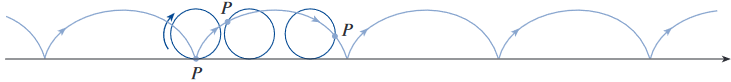
\includegraphics[scale=0.7]{cicloide.png}
\caption{Stewart, J (2017). \textit{Cálculo. Trascendentes Tempranas}. Pp. 643.}
\end{figure}

Para trazar la cicloide tenemos que conocer la \textbf{posición del punto} mientras rueda el círculo. Esto es posible de obtener usando \textbf{ecuaciones paramétricas}.

Digamos que tenemos un círculo de radio $r = a$ con centro $B$ y un punto $P$ en su circunferencia, el cual está rodando a una rapidez constante a lo largo del eje $x$ del plano cartesiano\footnote{Si fuese un camino, sería uno sin irregularidades o totalmente plano.}, donde $A$ es el punto donde toca dicho lugar.

\newpage

\begin{figure}[hbt!]
\centering

\begin{tikzpicture}
% Celdas de ayuda.
%\draw[help lines] (-7, -3) grid (7, 3);

% Ejes.
\draw[-latex, line width = 0.4mm] (-4.5, -2) -- (5, -2) node [below]{$x$};
\draw[-latex, line width = 0.4mm] (-4.5, -2) -- (-4.5, 2) node [left]{$y$};

% Radio circulo.
\draw (-2, -2) -- (-2, -0.5);
\node at (-2, -1.25) [right] {$a$};

% Linea con que se forma el angulo \theta.
\draw [dashed] (-2, -0.5) -- (-3.48, -0.7);
\node at (-2.5, -1) {$\theta$};

% Circulo (con el centro marcado con una X).
\draw (-2, -0.5) circle (1.5cm); % la coordenada (-2, -0.5) es el centro del circulo.
\draw [fill=black] (-2, -0.5) node [above]{$B$} circle (0.8mm);
\draw [fill=black] (-2, -2) node [below]{$A$} circle (0.8mm);

% Punto P.
\draw [fill=black] (-3.48, -0.7) circle (0.8mm);
\node at (-3.7, -0.4) {$P$};

% Origen.
\node at (-4.7, -1.8) {$0$};

% Efecto de movimiento del circulo.
\draw [->, line width=0.3mm] (-2.5, 1.2) arc (125:75:1cm);

\end{tikzpicture}

\end{figure}

Para conocer las ecuaciones paramétricas de $P$, usaremos el ángulo $\theta$ que se forma entre los radios $\overline{AB}$ y $\overline{PB}$, puesto que es la variable que indica mejor la posición de este punto mientras rueda el círculo.
\[
  P = (x(\theta), \ y(\theta))
\]
En cuanto a las ecuaciones de $x(\theta)$ e $y(\theta)$, se obtendrán mediante los componentes del vector $\overvec{OP}$ que resulta de la suma entre $\overvec{OA}$, $\overvec{AB}$ y $\overvec{BP}$, con $O$ siendo el origen.
\[
  \overvec{OP} = \overvec{OA} + \overvec{AB} + \overvec{BP}
\]
Geométricamente, nos estamos refiriendo a lo siguiente:

\begin{figure}[hbt!]
\centering

\begin{tikzpicture}
% Celdas de ayuda.
%\draw[help lines] (-7, -3) grid (7, 3);

% Ejes.
\draw[-latex, line width = 0.4mm] (-4.5, -2) -- (5, -2) node [below]{$x$};
\draw[-latex, line width = 0.4mm] (-4.5, -2) -- (-4.5, 2) node [left]{$y$};

% Radio circulo.
\node at (-2, -1.25) [right] {$a$};

% Linea con que se forma el angulo \theta.
\node at (-2.5, -1) {$\theta$};

% Circulo (con el centro marcado con una X).
\draw (-2, -0.5) circle (1.5cm); % la coordenada (-2, -0.5) es el centro del circulo.
\draw [fill=black] (-2, -0.5) node [above]{$B$} circle (0.8mm);
\draw [fill=black] (-2, -2) node [below]{$A$} circle (0.8mm);

% Punto P.
\draw [fill=black] (-3.48, -0.7) circle (0.8mm);
\node at (-3.7, -0.4) {$P$};

% Origen.
\node at (-4.7, -1.8) {$0$};

% Efecto de movimiento del circulo.
\draw [->, line width=0.3mm] (-2.5, 1.2) arc (125:75:1cm);

% Vectores
\draw [->, cyan, line width=0.5mm] (-4.5, -2) -- (-2, -2); % OA
\draw [->, cyan, line width=0.5mm] (-2, -2) -- (-2, -0.5); % AB
\draw [->, cyan, line width=0.5mm] (-2, -0.5) -- (-3.48, -0.7); % BP
\draw [->, red, line width=0.5mm] (-4.5, -2) -- (-3.48, -0.7); % OP

% Punto O.
\node at (-4.5, -2.25) {$O$};

\end{tikzpicture}

\end{figure}

Comencemos buscando los componentes de $\overvec{OA}$. Como el punto $A$ está tocando al eje $x$ mientras el círculo rueda a una rapidez constante, quiere decir que estuvo en el origen $O(0, \ 0)$. Por lo tanto, la distancia $d(OA) = |\overvec{OA}|$ será igual a la longitud del arco\footnote{La longitud del arco de un círculo corresponde al producto entre la fracción del ángulo que está subtendido del arco con respecto al ángulo del círculo completo (ambos en radianes) y la circunferencia de este último.\[\overline{AP} = \frac{\theta}{2 \pi} \cdot (2 \pi a) = a \cdot \theta\]} $\overline{AP}$.

\[
  \overline{AP} = d(OA) = |\overvec{OA}| = a \cdot \theta
\]
Y como $\overvec{OA}$ está horizontalmente en el eje $x$, entonces sus componentes son:
\[
  \overvec{OA} = \langle a \theta, \ 0 \rangle
\]
En cuanto a $\overvec{AB}$, como es paralelo a $y$ y su magnitud es igual al radio del círculo, podemos garantizar que sus componentes son:
\[
  \overvec{AB} = \langle 0, \ a \rangle
\]
Con respecto a $\overvec{BP}$, primero veamos que su magnitud es igual al radio del círculo, ya que comprende entre el centro $B$ y el punto $P$ que está en su circunferencia.
\[
  \left|\overvec{BP}\right| = a
\]
Además, entre $\overvec{BP}$ y parte de $\overvec{AB}$, junto con $\theta$, podemos formar un triángulo rectángulo.

\begin{figure}[hbt!]
\centering

\begin{tikzpicture}
%\draw [help lines] (-3, -3) grid (3, 3);

% Letra de los puntos.
\node at (1.2, 2.5) {$B$};
\node at (-2.4, 0.7) {$P$};
\node at (1.3, -1.5) {$A$};

% Puntos.
\draw [fill=black] (-2, 0.5) circle (0.8mm); % Punto P
\draw [fill=black] (1, 2.2) circle (0.8mm); % Punto B (centro del circulo)
\draw [fill=black] (1, -1.5) circle (0.8mm); % Punto A

\draw (-2, 0.5) -- (1, 0.5);
\draw [->, cyan, line width=0.5mm] (1, 2.2) -- (-2, 0.5); % Vector BP
\draw [->, cyan, line width=0.5mm] (1, -1.5) -- (1, 2.2); % Vector AB

% radio a.
\node at (-0.5, 1.6) {$a$};

\draw [dashed] (-3, 2.2) -- (3, 2.2);
\draw [dashed] (-2, 0.5) -- (-2, 2.2);
\draw [dashed] (1, 2.2) -- (1, 3);


% Angulos.
\node at (0.8, 1.8) {$\theta$};
\draw (1, 1) -- (0.5, 1) -- (0.5, 0.5);
\end{tikzpicture}

\end{figure}

Como podemos observar, a partir de los catetos del triángulo rectángulo de arriba podemos conocer los componentes de $\overrightarrow{BP}$ por medio de las funciones trigonométricas $\sin(\theta)$ y $\cos(\theta)$.
\begin{align*}
  \sin(\theta) &= \frac{\text{OP}}{a} & \cos(\theta) &= \frac{\text{ADY}}{a} \\
  a \cdot \sin(\theta) &= \text{OP} & a \cdot \cos(\theta) &= \text{ADY}
\end{align*}
Ahora bien, veamos que el ángulo $\theta$ está en el tercer cuadrante del plano cartesiano que se forma a partir del centro $B$ del círculo, por lo que los valores de OP y ADY serán negativos debido a que el $\sin(\theta) < 0$ y $\cos(\theta) < 0$ en dicho lugar. Por lo tanto:
\[
  \overvec{BP} = \langle -a \cdot \sin(\theta), \ -a \cdot \cos(\theta) \rangle
\]
Por consiguiente, los componentes de $\overrightarrow{OP}$ son:
\begin{align*}
  \overvec{OP} &= \langle a \theta, \ 0 \rangle + \langle 0, \ a \rangle + \langle -a \cdot \sin(\theta), \ -a \cdot \cos(\theta) \rangle \\
               &= \langle a \theta - a \sin(\theta), \ a - a \cos(\theta) \rangle
\end{align*}
y las ecuaciones paramétricas de $P$ con las cuales obtenemos la cicloide, son:
\[
  P = (a \theta - a \sin(\theta), \ a - a \cos(\theta))
\]
donde $\theta$ es el parámetro (varía) y $a$ el radio del círculo (se mantiene constante).

\end{document}
